


\chapter{Handouts}









This appendix contains materials that can be handed out as part of class activities (or repurposed
for other situations).

\newpage

\ 

\newpage

\section{What percentage of Earth is Covered with Water?}
\label{sec:googleMap}
You have probably heard that the Earth is 2/3 water, or 70\% water, or some other proportion
water.  How do people ``know'' this sort of stuff?  The answer is they don't ``know'' it, but
someone has estimated it.  Using the power of GoogleMaps, we can make our own estimate and see
if it is compatible with your folk knowledge.

%\subsection{Obtaining a Sample}
We can estimate the proportion of the world covered with water by randomly 
sampling points on the globe and inspecting them using GoogleMaps.


\begin{enumerate}
\item
First, let's do a sample size computation.  
If everyone in the class inspects 10 locations, what will our margin of error be?
\vspace{1in}
\vfill

\item
Suppose we want to estimate (at the usual 95\% confidence level) 
this proportion with $\pm 5$\%.  How large would our sample need to be?


\vspace{2in}

\item
Now fill in the following table.

\begin{center}
\large
\begin{tabular}{c|c}
\hline
margin of error & sample size \\
\hline
\hline
$\pm 5\%$ & \\[3mm]
$\pm 4\%$ & \\[3mm]
$\pm 2\%$ & \\[3mm]
$\pm 1\%$ & \\
\hline
\end{tabular}
\end{center}


\newpage
\item Generate enough random locations so that when we combine 
our data, we will get the precision we desire.  To do this, replace
the number \verb!10! with the appropriate value.

\begin{knitrout}
\definecolor{shadecolor}{rgb}{.97, .97, .97}{\color{fgcolor}\begin{kframe}
\begin{flushleft}
\ttfamily\noindent
\hlsymbol{positions}{\ }\hlassignement{\usebox{\hlnormalsizeboxlessthan}-}{\ }\hlfunctioncall{rgeo}\hlkeyword{(}\hlnumber{10}\hlkeyword{)}\mbox{}
\normalfont
\end{flushleft}
\begin{verbatim}
Error: could not find function "rgeo"
\end{verbatim}
\begin{flushleft}
\ttfamily\noindent
\hlsymbol{positions}\mbox{}
\normalfont
\end{flushleft}
\begin{verbatim}
Error: object 'positions' not found
\end{verbatim}
\end{kframe}}
\end{knitrout}


\item
Open a GoogleMap centered at each position.

\textbf{Turn off pop-up blocking for your default browser}, and then enter

\begin{knitrout}
\definecolor{shadecolor}{rgb}{.97, .97, .97}{\color{fgcolor}\begin{kframe}
\begin{flushleft}
\ttfamily\noindent
\hlfunctioncall{googleMap}\hlkeyword{(}\hlargument{pos}{\ }\hlargument{=}{\ }\hlsymbol{positions}\hlkeyword{,}{\ }\hlargument{mark}{\ }\hlargument{=}{\ }\hlnumber{TRUE}\hlkeyword{)}\mbox{}
\normalfont
\end{flushleft}
\end{kframe}}
\end{knitrout}


\item
For each map, record whether the center is located in water or on land.  \option{mark=TRUE}
is used to place a marker at the center of the map which is helpful for locations that are close to 
the coast.  
\begin{center}
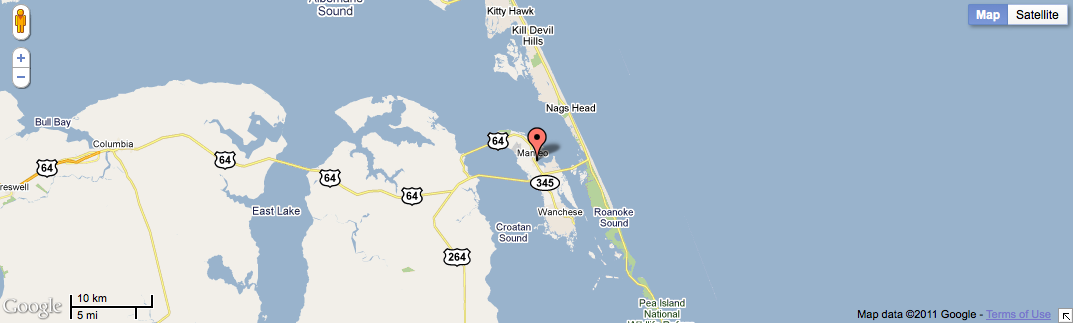
\includegraphics[width=.8\textwidth]{images/google-water1}
\end{center}
You can zoom in or out to get a better look.
\begin{center}
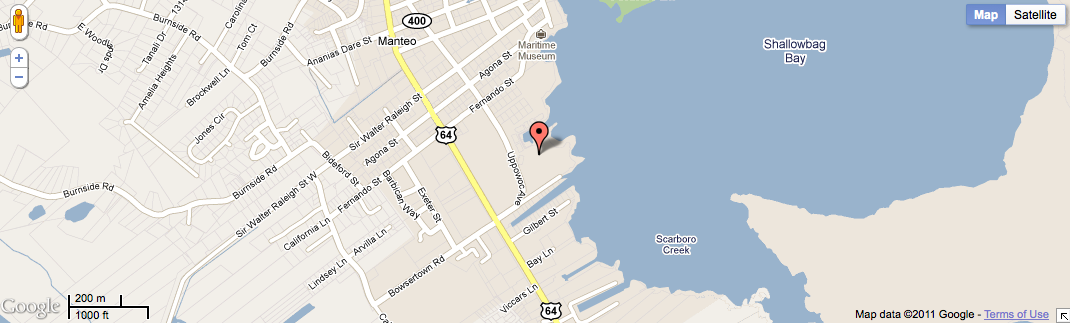
\includegraphics[width=.8\textwidth]{images/google-water2}
\end{center}


\item
Record your data in a GoogleForm at 

\begin{center}
\url{http://mosaic-web.org/uscots2011/google-water.html}
%https://spreadsheets.google.com/viewform?formkey=dGREcUR6YjRLSWFTWVpNNXA5ZUZ1TXc6MQ}

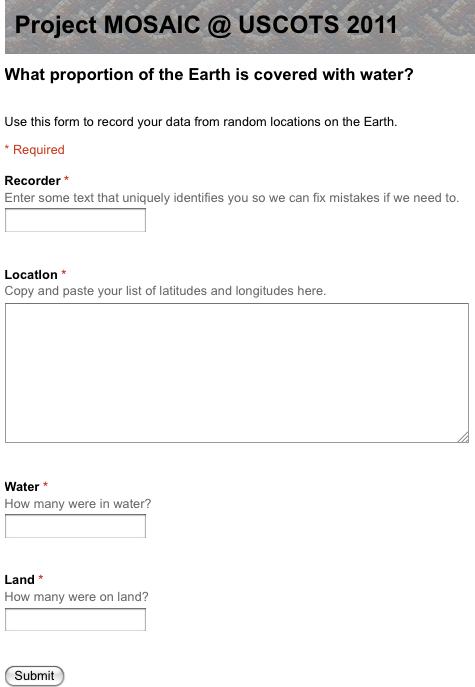
\includegraphics[width=.5\textwidth]{images/googleForm-water}
\end{center}

For the latitude and longitude information, simply copy and paste the output of 
\begin{knitrout}
\definecolor{shadecolor}{rgb}{.97, .97, .97}{\color{fgcolor}\begin{kframe}
\begin{flushleft}
\ttfamily\noindent
\hlsymbol{positions}\mbox{}
\normalfont
\end{flushleft}
\end{kframe}}
\end{knitrout}

\item
After everyone has entered their data into the GoogleForm,
grab the data from Google:

\begin{center}
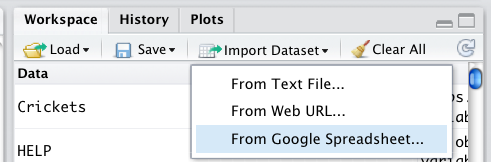
\includegraphics[width=4in]{images/google-spreadsheet1}
\end{center}


\item
Now it is simple to sum the counts across the class.
Here's how it turned out in a different class:




\begin{knitrout}
\definecolor{shadecolor}{rgb}{.97, .97, .97}{\color{fgcolor}\begin{kframe}
\begin{flushleft}
\ttfamily\noindent
\hlfunctioncall{sum}\hlkeyword{(}\hlsymbol{Water}\hlkeyword{\usebox{\hlnormalsizeboxdollar}}\hlsymbol{Water}\hlkeyword{)}\mbox{}
\normalfont
\end{flushleft}
\begin{verbatim}
[1] 215
\end{verbatim}
\begin{flushleft}
\ttfamily\noindent
\hlfunctioncall{sum}\hlkeyword{(}\hlsymbol{Water}\hlkeyword{\usebox{\hlnormalsizeboxdollar}}\hlsymbol{Land}\hlkeyword{)}\mbox{}
\normalfont
\end{flushleft}
\begin{verbatim}
[1] 85
\end{verbatim}
\end{kframe}}
\end{knitrout}


\item
Using our new data and your favorite analysis method (perhaps  \function{binom.test()})
give a 95\% confidence interval for the proportion of the world covered with water.

\vspace{1in}

\end{enumerate}


